\documentclass{article}
\usepackage{graphicx}
\graphicspath{ {/} }
\usepackage[utf8]{inputenc}
\usepackage[english]{babel}

\begin{document}
\section{Assignment 2}
\textbf{Question:}
Consider the prospects
\begin{equation}
A = (1, €3000), B = (0.8, €4000; 0.2, \$0), C = (0.25, €3000 0.75, 0), and D = (0.2, €4000; 0.8, 0).
\end{equation}
It has been found that most people prefer prospect A over prospect B and prospect D over prospect C. Show that Disappointment theory
as presented and parameterised in the book (p.100) can accommodate the observed choice pattern.


\textbf{Answer:}
\begin{equation}
L = (p_1: x_1, p_2: x_2, \ldots , p_n: x_n )
\end{equation}

\begin{equation}
DT(L) = \sum_i p_i [u(x_i) + D(u(x_i)- prior)]
\end{equation}

Assume liner utility $(U(x) = x)$, and:

- if outcome is above $EV, D=0.0002\times(x-EU)^2$
- if outcome is below $EV, D=0.0002\times(x-EU)^2$


\rule{\textwidth}{1pt}

\begin{flushleft}
\textbf{For A:}
\end{flushleft}
$EV=EU=3000$

$Prospect \hspace{2mm} A = 1 \times (3000 + 0.0002 \times (3000 - 3000)^2)) = 3000$

\\
\\

\begin{flushleft}
\color{red}
\textbf{For B:}
\end{flushleft}
$EV=EU=3200$

$Prospect \hspace{2mm} B = 0.8 \times (4000 + 0.0002 \times (4000 - 3200)^2)) + 0.2 \times (0 - 0.0002 \times (0 - 3200)^2)) = 2892,8$

\textbf{\textit{Hence:}} $Prospect \hspace{2mm} A > Prospect \hspace{2mm} B$

\rule{\textwidth}{1pt}

\begin{flushleft}
\textbf{For C:}
\end{flushleft}
$EV=EU=750$

$Prospect \hspace{2mm} C = 0.25 \times (3000 + 0.0002 \times (3000 - 750)^2)) + 0.75 \times (0 - 0.0002 \times (0 - 750)^2)) = 918,75$

\\
\\

\begin{flushleft}
\textbf{For D:}
\end{flushleft}
$EV=EU=800$

$Prospect \hspace{2mm} D = 0.2 \times (4000 + 0.0002 \times (4000 - 800)^2)) + 0.8 \times (0 - 0.0002 \times (0 - 800)^2)) = 1107,2$

\textbf{\textit{Hence:}} $Prospect \hspace{2mm} D > Prospect \hspace{2mm} C$

Hence, we conclude that disappointment theory can accommodate the observed choice pattern.


\begin{figure}
\centering
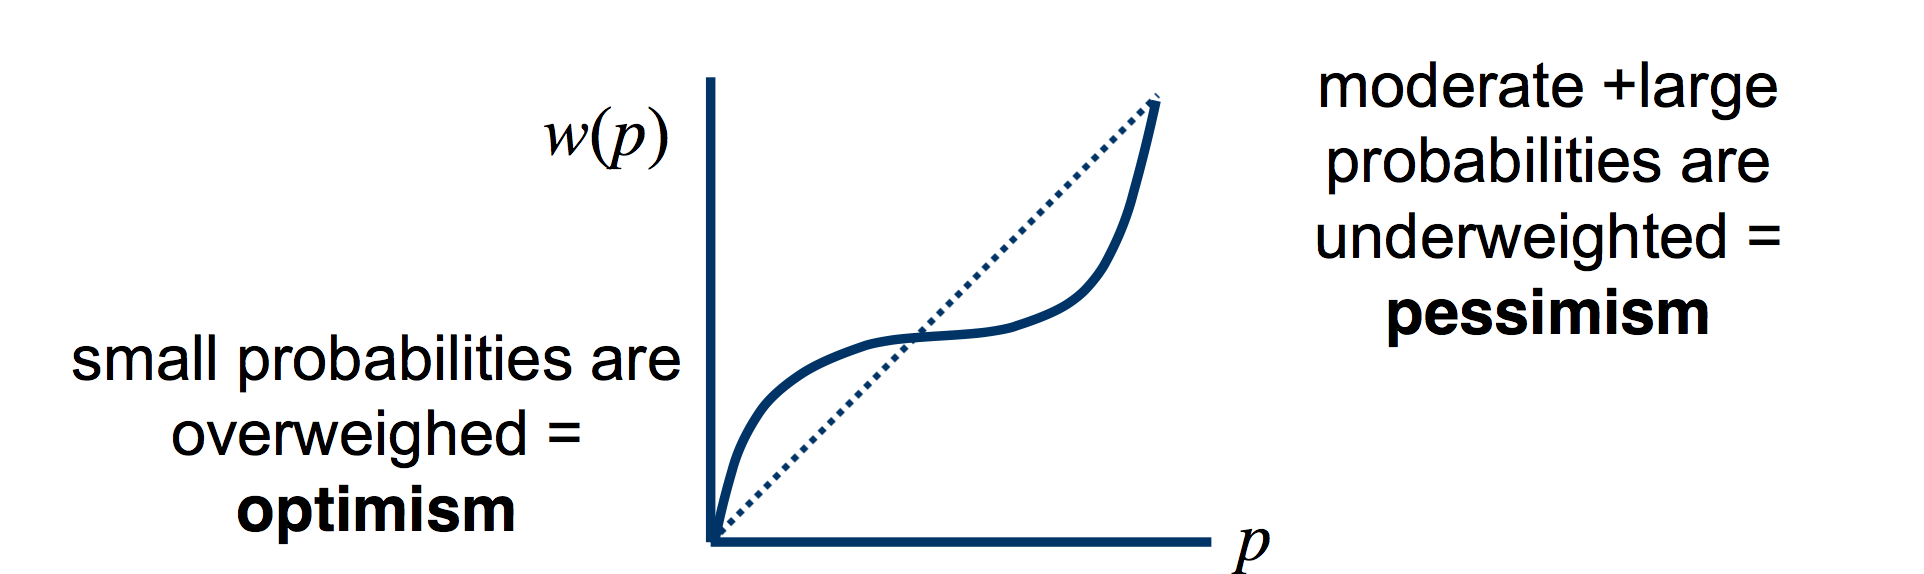
\includegraphics[width=20cm]{graph.png}
\end{figure}

\end{document}
